\documentclass[a4paper, twoside]{report}
\usepackage[margin=0.5in]{geometry}
\usepackage{amsmath}
\usepackage{amsfonts}
\usepackage{amssymb}
\usepackage{amsthm}
\usepackage{graphicx}
\usepackage{physics}
\usepackage{tikz}
\usepackage{mathrsfs}
\usepackage{pgfplots}
\usepgfplotslibrary{polar}
\usepgfplotslibrary{fillbetween}
\pgfplotsset{compat=1.18}
\usetikzlibrary{arrows,patterns, backgrounds, calc,fadings,shadows.blur, shapes}
\theoremstyle{plain}
\usepackage[most]{tcolorbox}
\usepackage{physunits}
\usepackage{float}
\usepackage[stable]{footmisc}
\usepackage{xcolor}
\usepackage{wrapfig}
\usepackage{microtype}
\usepackage{thmtools}
\usepackage[framemethod=TikZ]{mdframed}
\usepackage{steinmetz}
\usepackage{adjustbox}
\usepackage{listings}
\usepackage[version=4]{mhchem}
\newcommand{\floor}[1]{\lfloor #1 \rfloor}
\newcommand*{\Perm}[2]{{}^{#1}\!P_{#2}}%
\newcommand*{\Comb}[2]{{}^{#1}C_{#2}}%
\mdfsetup{skipabove=1em,skipbelow=0em}
\tcbuselibrary{xparse}
\usepackage[font=small,labelfont=bf,margin=\parindent,tableposition=top]{caption}
\newenvironment{solution}
{\renewcommand\qedsymbol{$\blacksquare$}\begin{proof}[Solution]}
	{\end{proof}}


\declaretheoremstyle[
headfont=\bfseries\sffamily\color{blue!70!black}, bodyfont=\normalfont,
mdframed={
	linewidth=2pt,
	rightline=false, topline=false, bottomline=false,
	linecolor=blue, backgroundcolor=blue!5,
}
]{thmbluebox}
\declaretheorem[style=thmbluebox, numbered=no, name=Example]{eg}


\declaretheoremstyle[
headfont=\bfseries\sffamily\color{blue!70!black}, bodyfont=\normalfont,
numbered=no,
mdframed={
	linewidth=2pt,
	rightline=false, topline=false, bottomline=false,
	linecolor=blue, backgroundcolor=blue!1,
},
]{thmexplanationbox}
\declaretheorem[style=thmexplanationbox, name=Solution]{tmpexplanation}
\newenvironment{explanation}[1][]{\vspace{-10pt}\begin{tmpexplanation}}{\end{tmpexplanation}}


\declaretheoremstyle[
headfont=\bfseries\sffamily\color{red!70!black}, bodyfont=\normalfont,
mdframed={
	linewidth=2pt,
	rightline=false, topline=false, bottomline=false,
	linecolor=red, backgroundcolor=red!5,
}
]{thmredbox}
\declaretheorem[style=thmredbox, name=Theorem]{theorem}

\declaretheoremstyle[
headfont=\bfseries\sffamily\color{red!70!black}, bodyfont=\normalfont,
numbered=no,
mdframed={
	linewidth=2pt,
	rightline=false, topline=false, bottomline=false,
	linecolor=red, backgroundcolor=red!2,
},
qed=\qedsymbol
]{thmproofbox}
\declaretheorem[style=thmproofbox, name=Proof]{replacementproof}
\renewenvironment{proof}[1][\proofname]{\vspace{-10pt}\begin{replacementproof}}{\end{replacementproof}}

\declaretheoremstyle[
headfont=\bfseries\sffamily\color{brown!70!black}, bodyfont=\normalfont,
mdframed={
	linewidth=2pt,
	rightline=false, topline=false, bottomline=false,
	linecolor=brown, backgroundcolor=brown!5,
}
]{thmbrownbox}
\declaretheorem[style=thmbrownbox, numbered=no, name=Question]{asign}

\declaretheoremstyle[
headfont=\bfseries\sffamily\color{brown!70!black}, bodyfont=\normalfont,
numbered=no,
mdframed={
	linewidth=2pt,
	rightline=false, topline=false, bottomline=false,
	linecolor=brown, backgroundcolor=brown!1,
},
]{thmansbox}
\declaretheorem[style=thmansbox, name=Answer]{thmbrown}
\newenvironment{anse}[1][]{\vspace{-10pt}\begin{thmbrown}}{\end{thmbrown}}

\tikzset {_uty0p60aj/.code = {\pgfsetadditionalshadetransform{ \pgftransformshift{\pgfpoint{0 bp } { 0 bp }  }  \pgftransformrotate{-270 }  \pgftransformscale{2 }  }}}
\pgfdeclarehorizontalshading{_zo7gli6ny}{150bp}{rgb(0bp)=(0.6,0.85,1);
rgb(53.66071428571429bp)=(0.6,0.85,1);
rgb(61.60714285714286bp)=(0,0.5,0.5);
rgb(100bp)=(0,0.5,0.5)}
\tikzset{every picture/.style={line width=0.75pt}} %set default line width to 0.75pt 

\usepackage[hidelinks]{hyperref}

\begin{document}
	\begin{titlepage}
			\begin{center}
			\Huge{Basics of Electronics and Communication Engineering (FCE0106)}\\
			Srijan Mahajan (2023UCM2326)\\
			Prof. Navneeta
		\end{center}
	\end{titlepage}
	\tableofcontents
	\newpage
	
	\chapter{Signals and Systems}

	A signal is defined as any physical quantity that varies with time, space, or any other independent variable or variables.
	
	The types of signals are: \begin{itemize}
		\item \textbf{ Continuous Time: }Represented as $x(t)$.
		\item \textbf{Discrete Time: }Represented as $x[n]$.
	\end{itemize}
	A system is an entity that processes a set of input signals to yield another set of output signals.
	\section{Elementary Functions}
	\subsection{Unit Step Function}
		\[u(t)=\begin{cases}
			1 &, t>0\\
			\frac{1}{2} &, t=0\\
			0&, t<0
			\end{cases}\]
			It is continuous for all $t$, except $t=0$. 
			\begin{figure}[H]
				\centering
				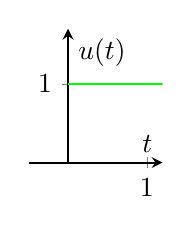
\begin{tikzpicture}
					\begin{axis}[
						x=1cm,y=1cm,
						axis lines=middle,
						xmin=-0.5,
						xmax=1.2,
						ymin=-0,
						ymax=1.7,
						xtick={-7,-6,...,10},
						ytick={-4,-3,...,5},
						ylabel={$u(t)$},
						xlabel={$t$},
						domain=0:2,
						samples=400,]
						\addplot[green, thick] {ifthenelse(x>0, 1, NaN)};
					\end{axis}
				\end{tikzpicture}
			\end{figure}
			In discrete time, it is defined as,
			\[u(n)=\begin{cases}
				1 &, n\geq0\\
				0 &, n<0
			\end{cases}\]

			\begin{figure}[h]
				\centering
				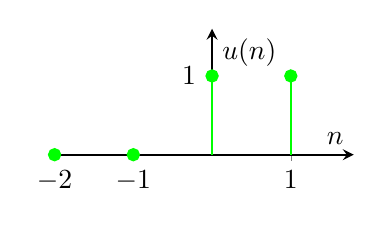
\begin{tikzpicture}
					\begin{axis}[
						x=1cm,y=1cm,
						axis lines=middle,
						xmin=-2,
						xmax=1.8,
						ymin=-0,
						ymax=1.6,
						xtick={-7,-6,...,10},
						ytick={-4,-3,...,5},
						ylabel={$u(n)$},
						xlabel={$n$},]
			\addplot+[ycomb,green,thick,mark=*,mark options={fill=green}] coordinates {(-2,0) (-1,0) (0,1) (1,1) (2,1)};
					\end{axis}
				\end{tikzpicture}
			\end{figure}
			\subsection{Unit Impulse Function}
			It is also called the Dirac Delta Function.
			\[\delta(t)=0 \; (t\neq0) \land \int\limits_{-\infty}^{\infty}\delta(t)\dd{t}=1\]
				\begin{figure}[h]
				\centering
				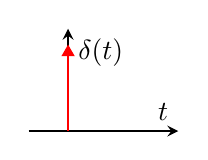
\begin{tikzpicture}
					\begin{axis}[
						x=1cm,y=1cm,
						axis lines=middle,
						xmin=-0.5,
						xmax=1.4,
						ymin=-0,
						ymax=1.3,
						xtick=\empty,
						ytick=\empty,
						ylabel={$\delta(t)$},
						xlabel={$t$},]
\addplot+[ycomb,red,thick,mark=triangle*,mark options={red,fill=red}] coordinates {(0,1)};
					\end{axis}
				\end{tikzpicture}
			\end{figure}
			The Delta function has many properties which is useful in analysis of functions.
			\begin{theorem}[Sifting Property]
				\[\int\limits_{-\infty}^{\infty}x(t)\delta(t)\dd{t}=\eval{x(t)}_{0}=x(0)\]
			\end{theorem}
			\begin{proof}
				Since the function is non-zero only at $t=0$, we can say,
				\[\int\limits_{-\infty}^{\infty}x(t)\delta(t)\dd{t}=\int\limits_{-\infty}^{\infty}x(0)\delta(t)\dd{t}=x(0)\]
			\end{proof}
			\begin{theorem}[Another form]
				\[\int\limits_{t_1}^{t_2}x(t)\delta(t-t_0)\dd{t}=\begin{cases}
					x(t_0) &, t_1<t_0<t_2\\
					0 &, \text{otherwise}
				\end{cases}\]
				\[x(t)=\int\limits_{-\infty}^{\infty}x(\tau)\delta(t-\tau)\dd{\tau}\]
			\end{theorem}
			\begin{theorem}[Scaling Property]
				\[\delta(at)=\frac{1}{|a|}\delta(t)\]
			\end{theorem}
			From this it follows that $\delta$ is an even function.
			\begin{theorem}[Sampling Property]
				\[x(t)\delta(t-t_0)=x(t_0)\delta(t-t_0)\]
			\end{theorem}
			\begin{theorem}[Differentiation Property]
				\[\int\limits_{-\infty}^\infty x(t)\delta'(t)\dd{t}=-x'(0)\]
			\end{theorem}
			\begin{theorem}[Amplitude Reversal]
				\[t\delta'(t)=-\delta(t)\]
			\end{theorem}
			\begin{theorem}[Derivative of Impulse Functions]
				\[\dv{\delta(t)}{t}=\delta'(t)=0 \; (t\neq0)\]
				Where,
				\[\int\limits_{-\infty}^\infty\delta'(t)=0\]
			\end{theorem}
			\subsection{Discrete Time Unit Impulse Function}
			\[\delta(n)=\begin{cases}
				1 &, n=0\\
				0 &, n\neq0
			\end{cases}\]
			\begin{theorem}
				\[\delta(kn)=\delta(n)\]
			\end{theorem}
			\begin{theorem}
				\[\delta(n)=u(n)-u(n-1)\]
				Or,
				\[u(n)=\sum\limits_{k=0}^\infty \delta(n-k)=\sum\limits_{k=-\infty}^\infty \delta(k)\]
			\end{theorem}
			\begin{theorem}
				\[x(n)\delta(n-k)=x(k)\delta(n-k)\]
			\end{theorem}
		\subsection{Unit Ramp Function}
		\[r(t)=tu(t)=\begin{cases}
			t &, t\geq0\\
			0 &, t<0
		\end{cases}\]
				\begin{figure}[H]
				\centering
				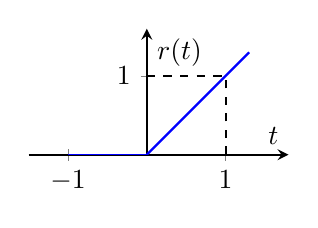
\begin{tikzpicture}
					\begin{axis}[
						x=1cm,y=1cm,
						axis lines=middle,
						xmin=-1.5,
						xmax=1.8,
						ymin=-0,
						ymax=1.6,
						xtick={-7,-6,...,10},
						ytick={-4,-3,...,5},
						ylabel={$r(t)$},
						xlabel={$t$},]
						\addplot[blue, thick, domain=0:1.3] {x};
						\addplot[blue, thick, domain=-1:0] {0};
						\draw[dashed] (axis cs:1,0) -- (axis cs:1,1);
						\draw[dashed] (axis cs:0,1) -- (axis cs:1,1);
					\end{axis}
				\end{tikzpicture}
			\end{figure}
		\begin{theorem}
			\[\dv{u(t)}{t}=\delta(t)\; \land \; \dv{r(t)}{t}=u(t)\]
		\end{theorem}
		In discrete time it is defined as
		\[r(n)=nu(n)\]
			\begin{figure}[h]
			\centering
			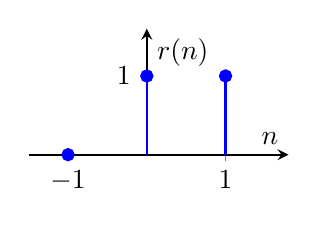
\begin{tikzpicture}
				\begin{axis}[
					x=1cm,y=1cm,
					axis lines=middle,
					xmin=-1.5,
					xmax=1.8,
					ymin=-0,
					ymax=1.6,
					xtick={-7,-6,...,10},
					ytick={-4,-3,...,5},
					ylabel={$r(n)$},
					xlabel={$n$},]
					\addplot+[ycomb,blue,thick,mark=*,mark options={blue,fill=blue}] coordinates {(-1,0) (0,1) (1,1) (2,1) (3,1)};
				\end{axis}
			\end{tikzpicture}
		\end{figure}
		\subsection{Real Exponential Signals}
		\[x(t)=Ce^{at}\]
		\begin{figure}[h]
			\centering
			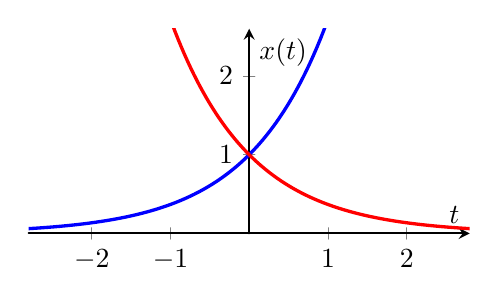
\begin{tikzpicture}[samples=250, line cap=round,line join=round,>=triangle 45,x=1cm,y=1cm]
				\begin{axis}[
					x=1cm,y=1cm,
					axis lines=middle,
					xmin=-2.8,
					xmax=2.8,
					ymin=-0,
					ymax=2.6,
					xtick={-7,-6,...,10},
					ytick={-4,-3,...,5},
					ylabel={$x(t)$},
					xlabel={$t$},]
					\addplot[very thick, blue] plot(\x,{exp(\x)});
					\addplot[very thick, red] plot(\x,{exp(-\x)});
				\end{axis}
			\end{tikzpicture}
			\caption*{\color{blue}$a>0$ \color{black}and \color{red} $a<0$}
		\end{figure}
		Similar results for discrete time exponential signals.
		\subsection{Complex Exponential Signals}
		\[x(t)=e^{j\omega_0 t}\]
		It has time period $\frac{2\pi}{|\omega_0|}$.
		\subsection{Signum Function}
		\[sgn(t)=\begin{cases}
			1 &, t>0\\
			0 &, t=0\\
			-1 &, t<0
		\end{cases}=2u(t)-1\]
		\subsection{Sampling Function}
		\[Sa(t)=\frac{\sin t}{t}\]
		To make the function continuous at $t=0$, we define $Sa(0)=1$.
		\[sinc(t)=\frac{\sin\pi t}{\pi t}=Sa(\pi t)\]
			\begin{figure}[h]
			\centering
			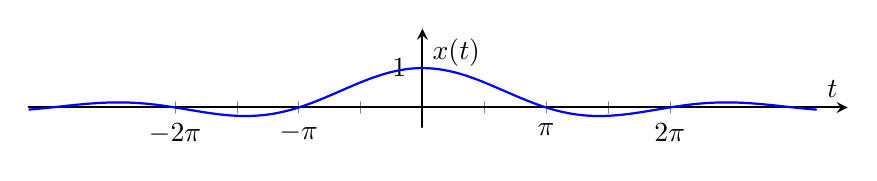
\begin{tikzpicture}[samples=500, line cap=round,line join=round,>=triangle 45,x=1cm,y=1cm]
				\begin{axis}[
					x=1cm,y=1cm,
					axis lines=middle,
					xmin=-10,
					xmax=10.8,
					ymin=-0.5,
					ymax=2,
					xtick={-2*pi, -(3/2)*pi, -pi, -(1/2)*pi, (1/2)*pi, pi, (3/2)*pi, 2*pi},
					xticklabels={$-2\pi$,,$-\pi$,,,$\pi$,,$2\pi$},
					ytick={-4,-3,...,1},
					ylabel={$x(t)$},
					xlabel={$t$},
					domain=-10:10,
					scale=0.5,]
					\addplot[blue, thick] {ifthenelse(x==0, 1, sin(deg(x))/x)};
				\end{axis}
			\end{tikzpicture}
		\end{figure}
		\section{Periodic and Aperiodic Signals}
		A signal is said to be periodic iff there exits $T$ such that,
		\[x(t+T)=x(t) \; \forall t\]
		Similarly for a discrete time signal,
		\[x(n+N)=x(n) \; \forall n\]
		\begin{theorem}
			\[\int\limits_a^{a+T} x(t)\dd{t}=\int\limits_b^{b+T} x(t)\dd{t} \; \forall a,b\]
		\end{theorem}
		\begin{theorem}
			A sum of $M$ periodic continuous time signals is periodic iff,
			\[\frac{T}{T_i}=n_i \quad 1\leq i\leq M\; \land n_i\in \mathbb{Z}\]
		\end{theorem}
		\section{Energy and Power Signals}
		The energy of a signal is given as,
		\[E_x=\int\limits_{-\infty}^\infty|x(t)|^2\dd{t} \; \text{OR} \; \sum\limits_{n=-\infty}^\infty |x(n)|^2\]
		The power of a signal is given as,
		\[P_x=\lim\limits_{T\to\infty}\frac{1}{T}\int\limits_{\frac{-T}{2}}^\frac{T}{2}|x(t)|^2\dd{t}=\lim\limits_{T\to\infty}\frac{1}{2T}\int\limits_{-T}^T|x(t)|^2\dd{t} \; \text{OR} \; \lim\limits_{N\to\infty}\frac{1}{2N+1}\sum\limits_{n=-N}^N |x(n)|^2\]
		A signal is said to be an energy signal if $E_x$ is finite and $P_x=0$. A signal is said to be a power signal\footnote{It is not practically possible to have a true power signal. All finite periodic signals are power signals.} if $P_x$ is finite and $E_x=\infty$.\\
		A signal cannot be an energy signal and power signal at the same time. But it is possible for a signal to be neither an energy signal or a power signal.
		\section{Even and Odd Signals}
		A signal is said to even when,
		\[x(-t)=x(t)\]
		A signal is said to be odd when,
		\[x(-t)=-x(t)\]
		Any given signal can be broken down into it's even and odd components.
		\[x(t)=\mathcal{E}\{x(t)\}+\mathcal{O}\{x(t)\}\]
		Where,
		\[\mathcal{E}\{x(t)\}=\frac{x(t)+x(-t)}{2} \; \land \; \mathcal{O}\{x(t)\}=\frac{x(t)-x(-t)}{2}\]
		\begin{theorem}[Multiplications]
			\[\begin{split}
				\text{Odd}\times\text{Odd} &=\text{Even}\\
				\text{Odd}\times\text{Even} &=\text{Odd}\\
				\text{Even}\times\text{Even} &=\text{Even}\\
			\end{split}\]			
		\end{theorem}
		\begin{theorem}[Derivatives]
			\[\begin{split}
				\dv{(\text{Even})}{t}&=\text{Odd}\\
				\dv{(\text{Odd})}{t}&=\text{Even}
			\end{split}\]
		\end{theorem}
		\section{Convolution}
		\subsection{Continuous Time Convolution}
		A convolution is an integral that expresses the amount of overlap of one function when it is shifted over another function.
		\[y(t)=(x\ast h)(t)=x(t)\ast h(t)=\int\limits_{-\infty}^\infty x(\tau)h(t-\tau)\dd{\tau}\]
		It is commutative, associative and distributive.
		\begin{theorem}[Time Shifting]
			\[x(t-t_1)\ast h(t-t_2)=t(t-t_1-t_2)\]
		\end{theorem}
		\begin{theorem}[Width Property]
			If the duration of $x$ and $h$ are finite and equal to $W_x$ and $W_h$, then the duration of the convolution is $W_x+W_h$.
		\end{theorem}
		\begin{theorem}[Differentiation Property]
			\[\left(\dv{t}x(t)\ast\right)h(t)=x(t)\ast\left(\dv{t}h(t)\right)=\dv{t}y(t)\]
		\end{theorem}
		\begin{theorem}[Time Scaling Property]
			\[x(at)\ast h(at)=\frac{1}{|a|}y(at)\]
		\end{theorem}
		\begin{theorem}[Even and Odd]
			\[\begin{split}
				\text{Odd}\ast\text{Odd} &=\text{Even}\\
				\text{Odd}\ast\text{Even} &=\text{Odd}\\
				\text{Even}\ast\text{Even} &=\text{Even}\\
			\end{split}\]
		\end{theorem}
		\begin{theorem}[Area Property]
			\[\int\limits_{-\infty}^\infty y(t)\dd{t}=\int\limits_{-\infty}^\infty x(t)\dd{t}\int\limits_{-\infty}^\infty h(t)\dd{t}\]
		\end{theorem}
		\subsection{Discrete Time Convolution}
		\[y(n)=x(n)\ast h(n)=\sum\limits_{k=-\infty}^\infty x(k)h(n-k)\]
		It is also commutative, associative and distributive. Similar properties like Time Shifting, Width Property, Sum Property\footnote{Analogous to Area Property} are similarly valid.
		\section{Continuous-Time Fourier Series}
		The Fourier Series allows us to represent any periodic signal as the sum of harmonically related sinusoidal functions.\\
		Any periodic signal can be expressed as a Fourier Series if it satisfies the Dirichlet conditions,
		\begin{itemize}
			\item if it is discontinuous, there are a finite number of discontinuities in the period $T$
			\item it has a finite average value over the period $T$
			\item it has a finite number of positive and negative maxima in the period $T$
		\end{itemize} 
		\subsection{Trigonometric Fourier Series}
		Any function $x$ satisfying Dirichlet conditions can be expressed as,
		\[x(t)=a_0+\sum\limits_{n=1}^\infty a_n\cos(n\omega_0 t)+b_n\sin(n\omega_0 t)\]
		Where the coefficients are given as,
		\[a_0=\frac{1}{T}\int\limits_0^T x(t)\dd{t} \; \land \; a_n=\frac{2}{T}\int\limits_0^Tx(t)\cos(n\omega_0t)\dd{t} \; \land \; b_n=\frac{2}{T}\int\limits_0^Tx(t)\sin(n\omega_0t)\dd{t}\]
		The integral may be carried over any full period.
		\begin{itemize}
			\item For any even function, $b_n=0$
			\item For any odd function, $a_0=0 \land a_n=0$
		\end{itemize}
		\begin{eg}
			Find the trigonometric Fourier Series for half-wave rectified sine wave.
			\begin{figure}[H]
				\centering
				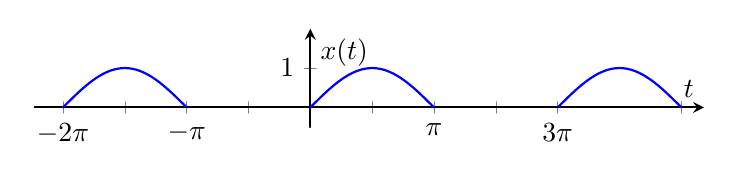
\begin{tikzpicture}[samples=500, line cap=round,line join=round,>=triangle 45,x=1cm,y=1cm]
					\begin{axis}[
						x=1cm,y=1cm,
						axis lines=middle,
						xmin=-7,
						xmax=10.0,
						ymin=-0.5,
						ymax=2,
						xtick={-2*pi, -(3/2)*pi, -pi, -(1/2)*pi, (1/2)*pi, pi, (3/2)*pi, 2*pi, 3*pi},
						xticklabels={$-2\pi$,,$-\pi$,,,$\pi$,,$3\pi$},
						ytick={-4,-3,...,1},
						ylabel={$x(t)$},
						xlabel={$t$},
						domain=-10:10,
						scale=0.5,]
						\addplot[blue, thick, domain=0:pi] {sin(deg(x))};
						\addplot[blue, thick, domain=2*pi:3*pi] {sin(deg(x))};
						\addplot[blue, thick, domain=-2*pi:-pi] {sin(deg(x))};
					\end{axis}
				\end{tikzpicture}
			\end{figure}
		\end{eg}
		\begin{explanation}
			Clearly, $T=2\pi \implies \omega_0=1$. Moreover, $x$ can be represented as,
			\[x(t)=\begin{cases}
				\sin t &, 0<t<\pi\\
				0 &, \pi <t < 2\pi
			\end{cases}\]
			Now, calculating the Fourier coefficients,
			\[a_0=\frac{1}{2\pi}\int\limits_0^{2\pi}\sin t\dd{t}=\frac{1}{2\pi}\int\limits_0^{\pi}\sin t\dd{t}=\frac{1}{\pi}\]
			\[\begin{split}
				a_n&=\frac{2}{2\pi}\int\limits_0^{\pi}\sin t\cos(nt)\dd{t}\\
				&=\frac{\cos(\pi n)+1}{\pi(1-n^2)}\\
				&=\begin{cases}
					0 &, n=3,5,\ldots\\
					\frac{2}{\pi (1-n^2)} &, n=2,4,\ldots
				\end{cases}
			\end{split}\]
			Clearly, at $n=1$,
			\[\lim\limits_{n\to 1}\frac{\cos(\pi n)+1}{\pi(1-n^2)}=0\implies a_1=0\]
			\[\begin{split}
				b_n&=\frac{2}{2\pi}\int\limits_0^{\pi}\sin t\sin(nt)\dd{t}\\
				&=\frac{\sin(n\pi)}{\pi(1-n^2)}\\
				&=0 \quad n\neq1
			\end{split}\]
			Clearly, at $n=1$,
			\[\lim\limits_{n\to 1}\frac{\sin(n\pi)}{\pi(1-n^2)}=0\implies b_1=\frac{1}{2}\]
			Now, for the line spectrum,
			\[c_0=\frac{1}{\pi} \; \land \; c_1=\frac{1}{2} \; \land \; c_n=|a_n| \; (\forall n\geq 2)\]
		\end{explanation}
		\subsection{Exponential Fourier Series}
		Any function $x$ satisfying Dirichlet conditions can be expressed as,
		\[x(t)=\sum\limits_{n=-\infty}^\infty X_n e^{jn\omega_0t}\]
		Where $X_n$ is given by,
		\[X_n=\frac{1}{T}\int\limits_0^T x(t)e^{-jn\omega_0t}\dd{t}\]
		\subsubsection{Relation between Trigonometric Fourier Series and Exponential Fourier Series}
		\[X_n=\frac{a_n-jb_n}{2}\; \land  \; X_{-n}=\frac{a_n+jb_n}{2}\]
		\begin{eg}
			Find the Exponential Fourier Series for half-wave rectified sine wave.
			\begin{figure}[H]
				\centering
				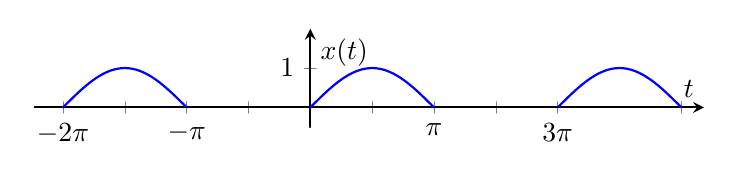
\begin{tikzpicture}[samples=500, line cap=round,line join=round,>=triangle 45,x=1cm,y=1cm]
					\begin{axis}[
						x=1cm,y=1cm,
						axis lines=middle,
						xmin=-7,
						xmax=10.0,
						ymin=-0.5,
						ymax=2,
						xtick={-2*pi, -(3/2)*pi, -pi, -(1/2)*pi, (1/2)*pi, pi, (3/2)*pi, 2*pi, 3*pi},
						xticklabels={$-2\pi$,,$-\pi$,,,$\pi$,,$3\pi$},
						ytick={-4,-3,...,1},
						ylabel={$x(t)$},
						xlabel={$t$},
						domain=-10:10,
						scale=0.5,]
						\addplot[blue, thick, domain=0:pi] {sin(deg(x))};
						\addplot[blue, thick, domain=2*pi:3*pi] {sin(deg(x))};
						\addplot[blue, thick, domain=-2*pi:-pi] {sin(deg(x))};
					\end{axis}
				\end{tikzpicture}
			\end{figure}
		\end{eg}
		\begin{explanation}
			Clearly, $T=2\pi \implies \omega_0=1$. Moreover, $x$ can be represented as,
			\[x(t)=\begin{cases}
				\sin t &, 0<t<\pi\\
				0 &, \pi <t < 2\pi
			\end{cases}\]
			Now, calculating the Fourier coefficients,
			\[\begin{split}
				X_n&=\frac{1}{2\pi}\int\limits_0^T \sin te^{-jnt}\dd{t}\\
				&=\frac{e^{-jn\pi}+1}{2\pi(1-n^2)}\\
				&=\begin{cases}
					\frac{1}{\pi(1-n^2)} &, n=0,\pm 2, \pm 4, \ldots\\
					0 &, n=\pm3,\pm5,\ldots
				\end{cases}
			\end{split}\]
			Clearly, at $n=\pm1$,
			\[\lim\limits_{n\to \pm1}\frac{e^{-jn\pi}+1}{2\pi(1-n^2)}=\frac{\mp j}{4}\]
		\end{explanation}
		\begin{theorem}[Time Shifting]
			\[x(t-t_0) \leftrightarrow e^{-jn\omega_0 t_0}X_n\]
		\end{theorem}
		\begin{theorem}[Frequency Shifting]
			\[e^{jm\omega_0 t}x(t)\leftrightarrow X_{n-m}\]
		\end{theorem}
		\begin{theorem}[Time Reversal]
			\[x(-t)\leftrightarrow X_{-n}\]
		\end{theorem}
		\begin{theorem}[Time Scaling]
			\[x(at)\leftrightarrow X_n\]
		\end{theorem}
		\begin{theorem}[Periodic Convolution]
			The periodic convolution of two periodic signals with same period is defined by,
			\[x(t)\circledast y(t)=\frac{1}{T}\int\limits_0^T x(\tau)y(t-\tau)\dd{\tau}\]
			Then, we can say that,
			\[x(t)\circledast y(t) \leftrightarrow X_nY_n\]
		\end{theorem}
		\begin{theorem}[Multiplication]
			\[x(t)y(t)\leftrightarrow \sum\limits_{k=-\infty}^\infty X_kY_{n-k}\]
		\end{theorem}
		\begin{theorem}[Differentiation]
			\[\dv[m]{x(t)}{t}\leftrightarrow (jn\omega_0)^mX_n\]
		\end{theorem}
		\begin{theorem}[Integration]
			\[\int\limits_{-\infty}^t x(t)\dd{t}\leftrightarrow \frac{1}{jn\omega_0}X_n\]
		\end{theorem}
		\begin{theorem}[Parseval's Theorem for Power Signals]
			If $x(t)\leftrightarrow X_n$, then,
			\[\frac{1}{T}\int\limits_0^T |x(t)|^2\dd{t}=\sum\limits_{n=-\infty}^\infty|X_n|^2=X_0+2\sum\limits_{n=1}^\infty|X_n|^2\]
			The theorem states that the total average power in a periodic signal equals the sum of the average powers in all of its harmonic components.
		\end{theorem}
		\begin{proof}
			\[\begin{split}
				\frac{1}{T}\int\limits_0^T |x(t)|^2\dd{t}&=\int\limits_0^T x(t)x^*(t)\dd{t}\\
				&=\int\limits_0^T x(t) \left(\sum\limits_{n=-\infty}^\infty X_ne^{jn\omega_0t}\right)^* \dd{t}\\
				&=\int\limits_0^T x(t) \left(\sum\limits_{n=-\infty}^\infty X^*_ne^{-jn\omega_0t}\right) \dd{t}\\
				&=\sum\limits_{n=-\infty}^\infty X^*_n\left(\frac{1}{T}\int_0^Tx(t)e^{-jn\omega_0t}\dd{t}\right)\\
				&=\sum\limits_{n=-\infty}^\infty X_n X^*_n\\
				&=\sum\limits_{n=-\infty}^\infty|X_n|^2
			\end{split}\]
		\end{proof}
		\section{Discrete-Time Fourier Series}
		Any function $x$ can be expressed as,
		\[x(n)=\sum\limits_{k=k_0}^{k_0+N-1}X_ke^{jk\omega_0 n}=\sum\limits_{k=<N>}X_ke^{jk\omega_0 n}\]\footnote{Here, $\sum\limits_{k=<N>}$ represents sum over any range of consecutive $k$'s of length $N$.}
		Where $X_k$ is given by,
		\[X_k=\frac{1}{N}\sum\limits_{n=<N>}x(n)e^{-jk\omega_0 n}\]
		\begin{theorem}[Time Shifting]
			\[x(n-n_0) \leftrightarrow e^{-jk\omega_0 n_0}X_k\]
		\end{theorem}
		\begin{theorem}[Frequency Shifting]
			\[e^{jM\omega_0 n}x(n)\leftrightarrow X_{k-M}\]
		\end{theorem}
		\begin{theorem}[Time Reversal]
			\[x(-n)\leftrightarrow X_{-k}\]
		\end{theorem}
		\begin{theorem}[Periodic Convolution]
			The periodic convolution of two periodic signals with same period is defined by,
			\[x(n)\circledast y(n)=\sum\limits_{r=<N>} x(r)y(n-r)\]
			Then, we can say that,
			\[x(n)\circledast y(n) \leftrightarrow NX_kY_k\]
		\end{theorem}
		\begin{theorem}[Multiplication]
			\[x(n)y(n)\leftrightarrow \sum\limits_{r=<N>} X_rY_{k-r}\]
		\end{theorem}
		\begin{theorem}[First Difference]
			\[x(n)-x(n-1)\leftrightarrow (1-e^{-jk\omega_0})X_k\]
		\end{theorem}
		\begin{theorem}[Running Sum/Accumulation]
			\[\sum\limits_{k=-\infty}^n x(k) \leftrightarrow \frac{X_k}{1-e^{-jk\omega_0}}\]
		\end{theorem}
			\begin{theorem}[Parseval's Relation]
			If $x(n)\leftrightarrow X_k$, then,
			\[\frac{1}{N}\sum\limits_{n=<N>} |x(n)|^2=\sum\limits_{k=<N>}|X_k|^2\]
			The theorem states that the total average power in a periodic signal equals the sum of the average powers in all of its harmonic components.
		\end{theorem}
		\begin{proof}
			\[\begin{split}
				\frac{1}{N}\sum\limits_{n=<N>} |x(n)|^2&=\frac{1}{N}\sum\limits_{n=<N>} x(n)x^*(n)\\
				&=\frac{1}{N}\sum\limits_{n=<N>} x(n)\left(\sum\limits_{k=<N>}X_ke^{jk\omega_0n}\right)^*\\
				&=\sum\limits_{k=<N>}X^*_k\left(\frac{1}{N}\sum\limits_{n=<N>}x(n)e^{-jk\omega_0n}\right)\\
				&=\sum\limits_{k=<N>}X_kX^*_k\\
				&=\sum\limits_{k=<N>}|X_k|^2
			\end{split}\]
		\end{proof}
		\section{Continuous Time Fourier Transform}
		The Fourier Transform of $x$ is given by,
		\[X(\omega)=\int\limits_{-\infty}^\infty x(t)e^{-j\omega t}\dd{t}\]
		And the inverse Fourier Transform of $X$ is given by,
		\[x(t)=\frac{1}{2\pi}\int\limits_{-\infty}^\infty X(\omega)e^{j\omega t}\dd{\omega}\]
		\begin{theorem}[Time Shifting]
			\[x(t-t_0)\leftrightarrow e^{-j\omega t_0}X(\omega)\]
		\end{theorem}
		\begin{theorem}[Frequency Shifting]
			\[x(t)e^{j\omega_0 t}\leftrightarrow X(\omega-\omega_0)\]
		\end{theorem}
		\begin{theorem}[Time and Frequency Scaling]
			\[x(at)\leftrightarrow \frac{1}{|a|}X\left(\frac{\omega}{a}\right)\]
		\end{theorem}
		\begin{theorem}[Area under $x(t)$]
			\[\int\limits_{-\infty}^\infty x(t)\dd{t}=X(0)\]
		\end{theorem}
		\begin{theorem}[Area under $X(\omega)$]
			\[\int\limits_{-\infty}^\infty X(\omega)\dd{\omega}=2\pi x(0)\]
		\end{theorem}
		\begin{theorem}[Differentiation in Time Domain]
			\[\dv[n]{x(t)}{t}\leftrightarrow (j\omega)^nX(\omega)\]
		\end{theorem}
		\begin{theorem}[Integration in Time Domain]
			\[\int\limits_{-\infty}^t x(\tau)\dd{\tau}\leftrightarrow \frac{X(\omega)}{j\omega}+\pi X(0)\delta(\omega)\]
		\end{theorem}
		\begin{theorem}[Differentiation in Frequency Domain]
			\[t^nx(t)\leftrightarrow j^n\dv[n]{X(\omega)}{\omega}\]
		\end{theorem}
		\begin{theorem}[Convolution Property]
			\[x(t)\ast y(t)\leftrightarrow X(\omega)Y(\omega)\]
		\end{theorem}
		\begin{theorem}
			\[x(t)y(t)\leftrightarrow \frac{1}{2\pi}\left[X(\omega)\ast Y(\omega)\right]\]
		\end{theorem}
		\begin{theorem}[Duality]
			\[X(t)\leftrightarrow 2\pi x(-\omega)\]
		\end{theorem}
		\begin{theorem}[Parseval's Relation]
			\[E_x=\int\limits_{-\infty}^\infty |x(t)|^2\dd{t}=\frac{1}{2\pi}\int\limits_{-\infty}^\infty |X(\omega)|^2\dd{\omega}\]
		\end{theorem}
		\subsection{Fourier Transform of Elementary Functions}
		\begin{eg}[D.C. Value]
			\[x(t)=A_0\]
		\end{eg}
		\begin{explanation}
			Let there be a function $X(\omega)=A_0\delta(\omega)$, which is the Fourier Transform of $x(t)$, 
			\[\begin{split}
				x(t)&=\frac{1}{2\pi}\int\limits_{-\infty}^\infty X(\omega)e^{j\omega t}\dd{\omega}\\
				\therefore x(t)&=\frac{A_0}{2\pi}
			\end{split}\]
			Thus, 
			\[\mathcal{F} \left\{\frac{A_0}{2\pi}\right\}=A_0\delta(\omega) \implies \mathcal{F}\{A_0\}=2\pi A_0\delta(\omega)\]
		\end{explanation}
		\begin{eg}[Impulse Function]
			\[x(t)=\delta(\omega)\]
		\end{eg}
		\begin{explanation}
			\[\begin{split}
				X(\omega)&=\int\limits_{-\infty}^\infty \delta(t)e^{-j\omega t}\dd{t}\\
				\therefore X(\omega)&=1
			\end{split}\]
			Thus,
			\[\mathcal{F}\left\{\delta(t)\right\}=1\]
		\end{explanation}
		\begin{eg}[Exponential]
			\[x(t)=e^{-at}u(t)\]
		\end{eg}
		\begin{explanation}
			\[\begin{split}
				X(\omega)&=\int\limits_{0}^\infty e^{-at}e^{-j\omega t}\dd{t}\\
				&=\frac{1}{a+j\omega}
			\end{split}\]
			Thus,
			\[\mathcal{F}\left\{e^{-at}u(t)\right\}=\frac{1}{a+j\omega}\]
		\end{explanation}
		\begin{eg}[Exponential]
			\[x(t)=e^{-a|t|}\]
		\end{eg}
		\begin{explanation}
			\[\begin{split}
				X(\omega)&=\int\limits_{-\infty}^0 e^{at}e^{-j\omega t}\dd{t}+\int\limits_{0}^\infty e^{-at}e^{-j\omega t}\dd{t}\\
				&=\frac{1}{a-j\omega}+\frac{1}{a+j\omega}\\
				&=\frac{2a}{a^2+\omega^2}
			\end{split}\]
			Thus,
			\[\mathcal{F}\left\{e^{-a|t|}\right\}=\frac{2a}{a^2+\omega^2}\]
		\end{explanation}
		\begin{eg}[Signum Function]
			\[x(t)=sgn(t)\]
		\end{eg}
		\begin{explanation}
			Simplifying the function
			\[x(t)=u(t)-u(-t)=\lim\limits_{a\to 0}e^{-at}u(t)-e^{at}u(-t)\]
			\[\begin{split}
				X(\omega)&=\lim\limits_{a\to0}\frac{1}{a+j\omega} - \frac{1}{a-j\omega}\\
				&=\frac{2}{j\omega}
			\end{split}\]
			Thus,
			\[\mathcal{F}\left\{sgn(t)\right\}=\frac{2}{j\omega}\]
		\end{explanation}
		\begin{eg}[Unit Step Function]
			\[x(t)=u(t)\]
		\end{eg}
		\begin{explanation}
			\[x(t)=\frac{1}{2}+\frac{sgn(t)}{2}\]
			\[\begin{split}
				X(\omega)&=2\pi\left(\frac{1}{2}\right)\delta(\omega)+\frac{1}{2}\frac{2}{j\omega}\\
				&=\frac{1}{j\omega}+\pi\delta(\omega)
			\end{split}\]
			Thus,
			\[\mathcal{F}\left\{u(t)\right\}=\frac{1}{j\omega}+\pi\delta(\omega)\]
		\end{explanation}
		\begin{eg}[Complex Exponential Signal]
			\[x(t)=e^{j\omega_0 t}\]
		\end{eg}
		\begin{explanation}
			Consider the D.C. value $1$,
			\[\mathcal{F}\left\{1\right\}=2\pi\delta(\omega)\implies \mathcal{F}\left\{e^{j\omega_0 t}\right\}=2\pi\delta(\omega-\omega_0) \quad (\text{Frequency Shifting})\]
		\end{explanation}
		\begin{eg}[Cosine Function]
			\[x(t)=\cos\omega_0t\]
		\end{eg}
		\begin{explanation}
			\[x(t)=\frac{e^{j\omega_0t}+e^{-j\omega_0t}}{2}\]
			Thus,
			\[\mathcal{F}\left\{\cos\omega_0t\right\}=\pi\left[\delta(\omega-\omega_0)+\delta(\omega+\omega_0)\right]\]
		\end{explanation}
		\begin{eg}[Sine Function]
			\[x(t)=\cos\omega_0t\]
		\end{eg}
		\begin{explanation}
			\[x(t)=\frac{e^{j\omega_0t}-e^{-j\omega_0t}}{2}\]
			Thus,
			\[\mathcal{F}\left\{\sin\omega_0t\right\}=\pi\left[\delta(\omega-\omega_0)-\delta(\omega+\omega_0)\right]\]
		\end{explanation}
		\begin{eg}[Rectangular Function]
			\[x(t)=A\text{rect}\left(\frac{t}{\tau}\right)\]
		\end{eg}
		\begin{explanation}
			Here, we use the method of differentiation,
			\[\dv{t}x(t)=A\left[\delta(t+\frac{\tau}{2}) - \delta(t-\frac{\tau}{2})\right]\]
			Now using the Differentiation Property,
			\[(j\omega)X(\omega)=A\left[e^{j\omega\frac{\tau}{2}}-e^{-j\omega\frac{\tau}{2}} \right] \implies X(\omega)=\frac{A}{\omega}2\sin(\omega\frac{\tau}{2})\]
			Thus,
			\[\mathcal{F}\left\{ A\text{rect}\left(\frac{t}{\tau}\right) \right\}=\frac{A}{\omega}2\sin(\omega\frac{\tau}{2})=A\tau Sa\left(\omega\frac{\tau}{2}\right)\]
		\end{explanation}
		\begin{eg}[Sampling Function]
			\[x(t)=Sa(t)=\frac{\sin t}{t}\]
		\end{eg}
		\begin{explanation}
			Using the Duality Property,
			\[\mathcal{F}\left\{Sa(t)\right\}=\frac{\text{rect}\left(\frac{\omega}{2}\right)}{2}\]
		\end{explanation}
\end{document}